%%%%%%%%%%%%%%%%%%%%%%% file template.tex %%%%%%%%%%%%%%%%%%%%%%%%%
%
% This is a general template file for the LaTeX package SVJour3
% for Springer journals.          Springer Heidelberg 2010/09/16
%
% Copy it to a new file with a new name and use it as the basis
% for your article. Delete % signs as needed.
%
% This template includes a few options for different layouts and
% content for various journals. Please consult a previous issue of
% your journal as needed.
%
%%%%%%%%%%%%%%%%%%%%%%%%%%%%%%%%%%%%%%%%%%%%%%%%%%%%%%%%%%%%%%%%%%%

\RequirePackage{fix-cm}
%\documentclass[twocolumn]{svjour3}          % twocolumn
\documentclass[smallextended]{svjour3}          % twocolumn

\smartqed  % flush right qed marks, e.g. at end of proof

\usepackage{graphicx} % adjustbox loads it
\usepackage{epstopdf} % loads eps
\usepackage[normalem]{ulem}

% insert here the call for the packages your document requires
\usepackage{geometry}
\usepackage[export]{adjustbox}
\usepackage[labelfont=bf, labelsep=space]{caption}
%\usepackage{subcaption}
\usepackage{subfig}
\usepackage[utf8]{inputenc}
\usepackage{amssymb}
\usepackage{amsmath} 

\usepackage{natbib} % enables author year and other citation styles
\usepackage[bookmarks,bookmarksopen,bookmarksdepth=2]{hyperref} % active links
\hypersetup{backref,
	colorlinks=true,
	citecolor=blue,
	linkcolor=blue}

\usepackage{tikz} % graphics,
\usetikzlibrary{fit,positioning} % tikz elements positioning
\usepackage{soul} % annotations


\DeclareMathOperator*{\argmin}{arg\,min}

\newcommand\alberto[1]{\textcolor{red}{#1}}

%\DeclareGraphicsRule{.tif}{png}{.png}{`convert #1 `dirname #1`/`basename #1 .tif`.png}

\graphicspath{ {./img/} }
\DeclareMathOperator*{\argmax}{arg\,max}
\journalname{Comput Stat}

\begin{document}
\title{Structural posts neighborhoods to characterize users in online forums}

\author{Alberto Lumbreras \and
        Julien Velcin  \and\\
        Marie Guégan \and
        Bertrand Jouve
}

\institute{Alberto Lumbreras \and Marie Guégan \at
		   Technicolor\\
           975 Avenue des Champs Blancs, \\35576 Cesson-Sévigné,\\ France\\
           \email{alberto.lumbreras@technicolor.com}\\
           \email{marie.guegan@technicolor.com}
           \and
           Julien Velcin \at
           Laboratoire ERIC, Université de Lyon,\\
           5, avenue Pierre Mendès France, 69676 Bron,\\ France\\
           \email{julien.velcin@univ-lyon2.fr}
		  \and
           Bertrand Jouve \at
           Université de Toulouse; UT2; FRAMESPA/IMT; 5 allée Antonio Machado, 31058 Toulouse, cedex 9\\
           CNRS; FRAMESPA; F-31000 Toulouse\\
           CNRS; IMT; F-31000 Toulouse\\ France\\     
           \email{jouve@univ-tlse2.fr}
}

\date{Draft date: \today}
% The correct dates will be entered by the editor

\maketitle

%%%%%%%%%%%%%%%%%%%%%%%%%%%%%%%%%%%%%%%%%%%%%%%%%%%%%%
%%%%%%%%%%%%%%%%%%%%%%%%%%%%%%%%%%%%%%%%%%%%%%%%%%%%%%
\section{Introduction}\label{sec:introduction}

The popularization of online forums has brought a growing interest on their underlying dynamics. As any other complex system, an the dynamic of online forums can be studied at different levels, from the more macro to the most micro. Macro dynamics are, for instance, the evolution of some global properties such as its diameter, or its distribution degree. Micro dynamics are, for instance, the triadic motifs that represent local phenomena such as transitivity (friends of my friends are also my friends).

An interesting question in online communities is that concerning roles. In sociology, roles are generally seen as the set of expected behaviors that are attached  to a position in the community. Extrapoliting the notion of role, some researchers have looked for roles in online forums. Some others have tried to detect the roles and the users who hold that roles.

Roles can also be studied from the macro or the micro perspective. If studied from the macro, we can analyze the number of users, the percentage of replied post, its centrality in the network, and  so forth.

In this paper, we focus on the anamyse of roles at a micro level, and more specifically at the discussion level. We would like to answer the following question: are there different types of users in terms of the kind of conversation they participate in?

The remaining of the paper is as follows. First we will introduce our representation of online discussions. Then we will explain our concept of structural neighborhood. Then we will apply this to the clustering of users and we will analyze the clusters. Finally, we will attemp to study whether these roles have predictive power.


\section{Discussion trees}
A very natural way to represent a conversation thread is a tree graph where vertex represent posts and edges represent replies from some post to another. The tree is rooted at the post who started the thread. This representation allows to apply the mathematical toolbox of graph theory. Figure~\ref{fig:trees} shows some real examples of trees in a Reddit\footnote{www.reddit.com} forum.

\begin{figure}
	\centering
	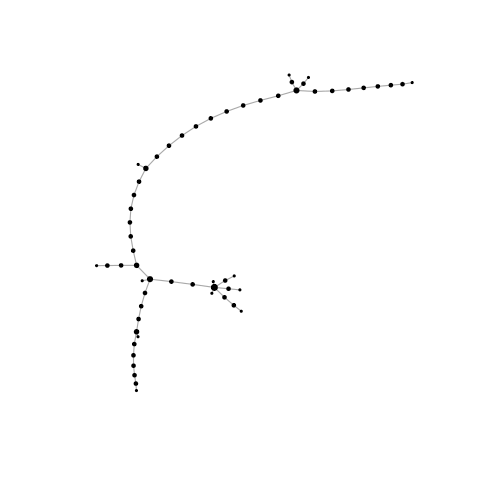
\includegraphics[width=0.32\textwidth]{tree1}
	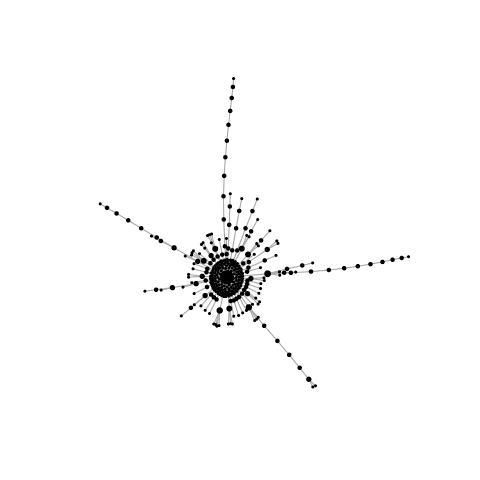
\includegraphics[width=0.32\textwidth]{tree2}
	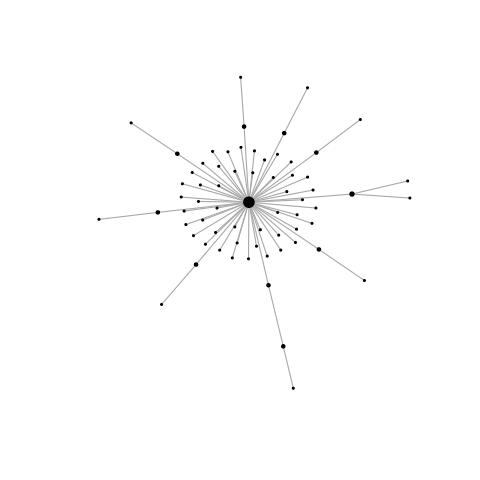
\includegraphics[width=0.32\textwidth]{tree3}
	\caption{Representation of discussion threads with post tree graphs. Vertex represent posts and edges represent replies between posts.}
	\label{fig:trees}
\end{figure}
\section{Posts graph neighborhoods}

Our intuition is that some users like participating in some kind of discussion rather than other. Certainly, an analysis of the textual content will tell us much about a discussion. However, due to the huge diversity of topics, vocabulary, and the difficulty of current algorithms to capture the language subtleties such as humor, irony, or changing contexts, we turn our attention towards the structure of the discussions. More precisely, we analyze the local graph structure in which a user post in embedded, in the hope that this structure will be meaningful since it also reflects the kind of conversation in that part of the thread.

Formally, these local graphs are known as neighborhoods. Let us consider first the most basic notion of neighborhood in order to understand its limitations. Let $p_i$ be a post in the tree graph $G$. The \textit{neighborhood of $p_i$ at radius $r$} $N_G(p_i,r)$ is the induced subgraph of $G$ consisting of all posts $j \in G$ at distance $d_{ij}\leq r$. In order to analyze the type of discussion where a user participates in, we might count the different neighborhoods in which her posts are embedded. However, the number of possible neighborhoods even with radius 1 is unbounded since, although a post can only have a parent, it can have an infinite number of children (see Figure~ \ref{fig:large_neighboorhood}). 

In practice, if we create a matrix $M$ where rows correspond to users, columns correspond to neighborhoods and $M_{ij}$ indicates how many times user $i$ has a post in the neighborhood $j$,  we obtain a very sparse matrix. Moreover, many of the columns correspond to similar type of neighborhoods. Think, for instance, of a post with 1 reply, a post with 10 replies and another post with 15 replies. While the type of conversation that embeds the first posts is different from the other two, it does not make sense to say that the former two are categorically different.

\begin{figure}
	\centering
	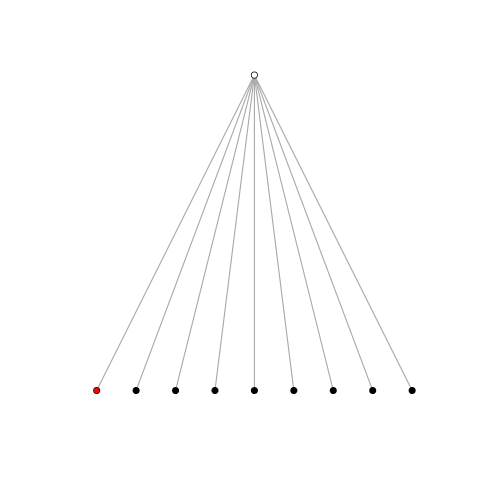
\includegraphics[width=0.4\textwidth]{large_neighborhood}
	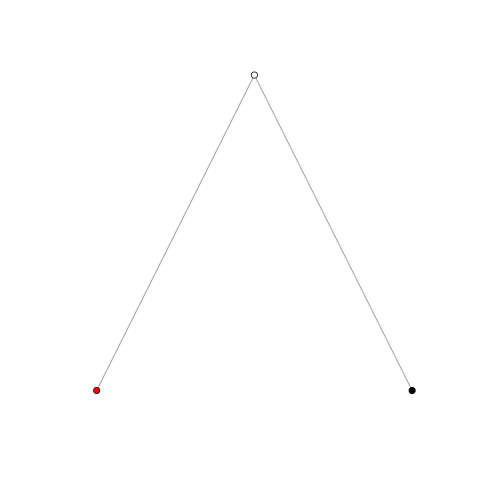
\includegraphics[width=0.4\textwidth]{small_neighborhood}
	\caption{The size of the neighborhood at distance $R$ is unbounded. These two graph represent frequent neighborhoods of a post (red) that replied to the root (white). However, the tree in the left corresponds to a very successful root while the three in the right has not brought the attention of too many users.}
	\label{fig:large_neighboorhood}
\end{figure}

In order to reduce the space of possible neighborhoods we introduce the notion of \textit{temporal neighborhood}. Let $t_i$ the time where post $p_i$ was added to the thread $G$. Let $\tau_{ij}=|t_i-t_j|$ be the \textit{temporal distance} between two posts $p_i$ and $p_j$. The \textit{temporal neighborhood} $N_{G}^{(t)}(i, r, n)$of spacial radius $r$ and order $n$ of a post $p_i$ is the set of $n$ posts in its spacial neighborhood $N_{G}(i, r)$ that are temporally closest to $i$ and that can reach $i$ trough posts that are also in the temporal neighborhood.

Finally, we give their own colors the post $i$ and to the root, and we consider that two neighborhoods are equivalent if they are color-isomorphic.

With the above definitions in mind, and for a given forum, we can build a matrix $M$ with the counts of neighborhoods for every user. 

\section{Application to Reddit forums}

We analyze the Podemos forum\footnote{https://www.reddit.com/r/podemos} in Reddit. It was was first used as a tool of internal democracy. Today, its members use it also to share and discuss about political news.
The Podemos forum contains 995 discussion threads that started on January. These threads contain a total of 12912 posts written by 1218 users.

\subsection{Counting neighorhoods}
In this section we will build a matrix $M$ for one of the forums of Reddit and then we will cluster users to find groups that have similar preferences over the different types of conversations represented by the neighborhood structures. 

If we set the a spatial radius $r=1$ and an order $n=4$, the temporal neighborhood $N_{G}^{(t)}(i, 1, 4)$ recovers the four adjacent posts that were written temporally closest to a given post. Figure~\ref{fig:neighborhoods_1_4} shows the four detected neighborhoods and their frequency.

In order to detect more complex types of neighborhoods we enlarge the spatial radius to $r=4$. Figure~\ref{fig:neighborhoods_4_4} shows the eight detected neighbors and their frequency. It is interesting to see different structures like chains or stars where the root node migh or might no appear and the ego post is placed at different positions.

\begin{figure}
	\centering
	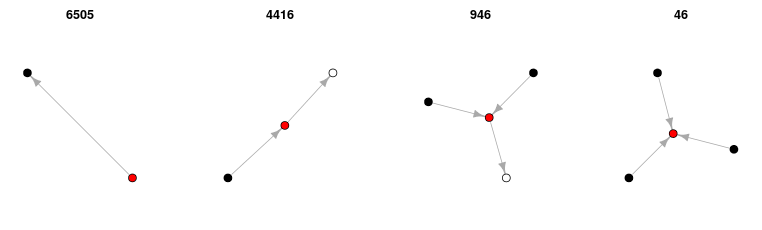
\includegraphics[width=0.8\textwidth]{neighborhoods_1_4}
	\caption{Neighborhood counts with $r=1$ and $n=4$}
	\label{fig:neighborhoods_1_4}
\end{figure}

\begin{figure}
	\centering
	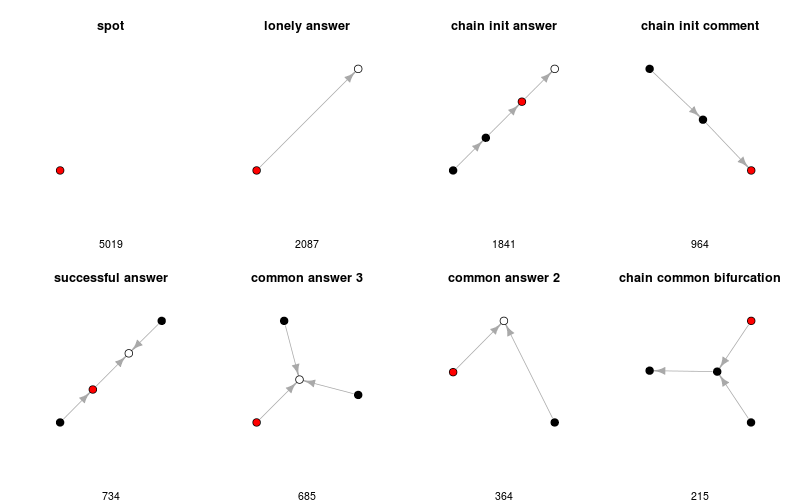
\includegraphics[width=0.8\textwidth]{neighborhoods_4_4}
	\caption{Neighborhood counts with $r=4$ and $n=4$}
	\label{fig:neighborhoods_4_4}
\end{figure}

Note that some neighbors are still very similar. For instance, \textit{common answer 3} is very close to \textit{common answer 2} in the sense that they both represent the ego post replying to a root post that has one and two replies respectively. It seems a good idea to merge them both since they seem to represent the same type of discussion.

\subsection{Clustering}

Given the neighborhoods in which each user participates, we will analyze whether there exists different types of users or all users look similar.

We want to make the analyze independent of the number of posts, and for that we normalize each user feature vector so that features indicate the percentage of posts in this kind of neighborhood. Moreover, some neighborhoods are much more common than others due to the nature of the forums. Thus, we normalize and scale the features so that every feature has a global mean 0 and variance 1. User features now represent z-scores, that is, how many standard deviations is this user feature away from the mean.

We use a simple k-means to find the clusters. To decide the number of clusters, we run k-means for k=2,...,25 clusters and look at the Within-Cluster Sum of Squares (Figure~\ref{fig:elbow}) and we chose $k=5$ so that the results are more interpretable.  Figure~\ref{fig:PCA} shows a PCA projection of the users colored by cluster and the distribution of the clusters in every dimension.
\begin{figure}
	\centering
	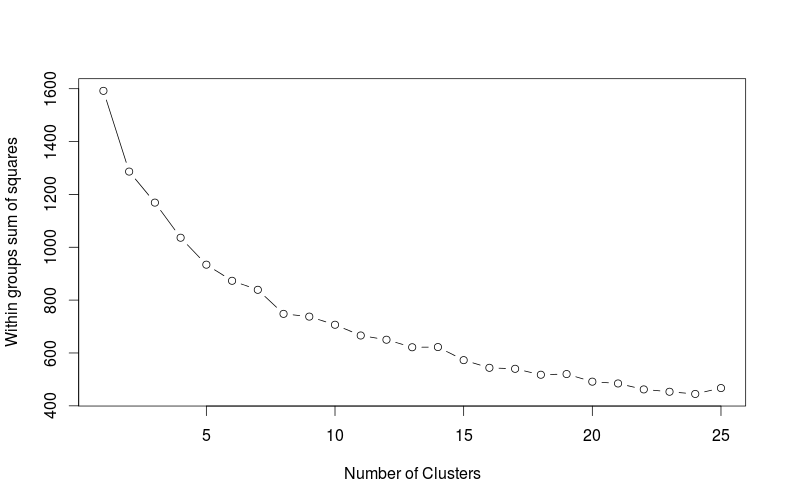
\includegraphics[width=0.5\textwidth]{elbow}
	\caption{Within-Sum of Squares under k-means}
	\label{fig:elbow}
\end{figure}

\begin{figure}
	\centering
	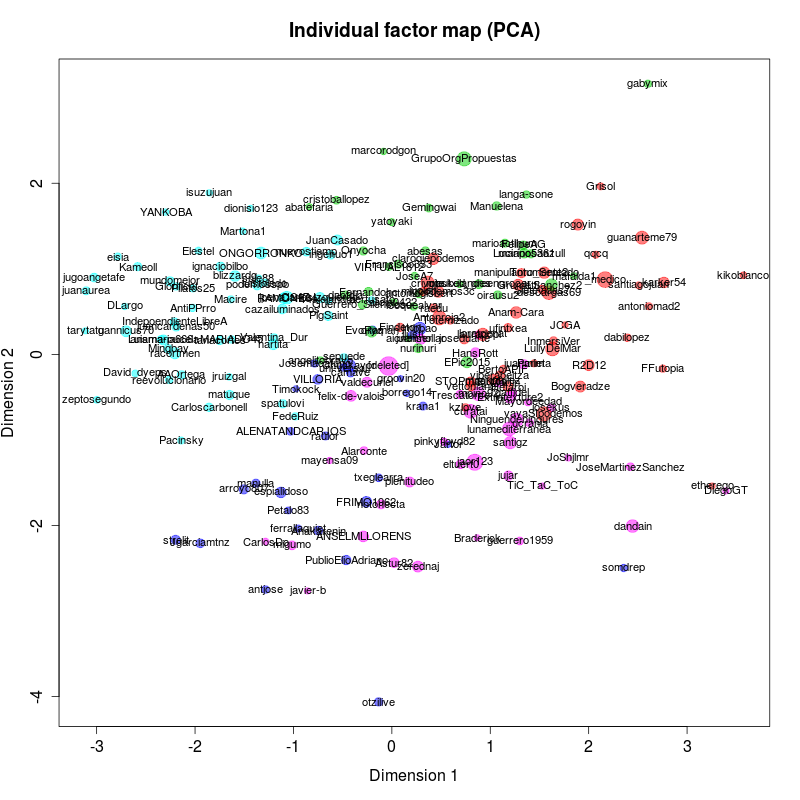
\includegraphics[width=0.5\textwidth]{PCA_nocolor}
	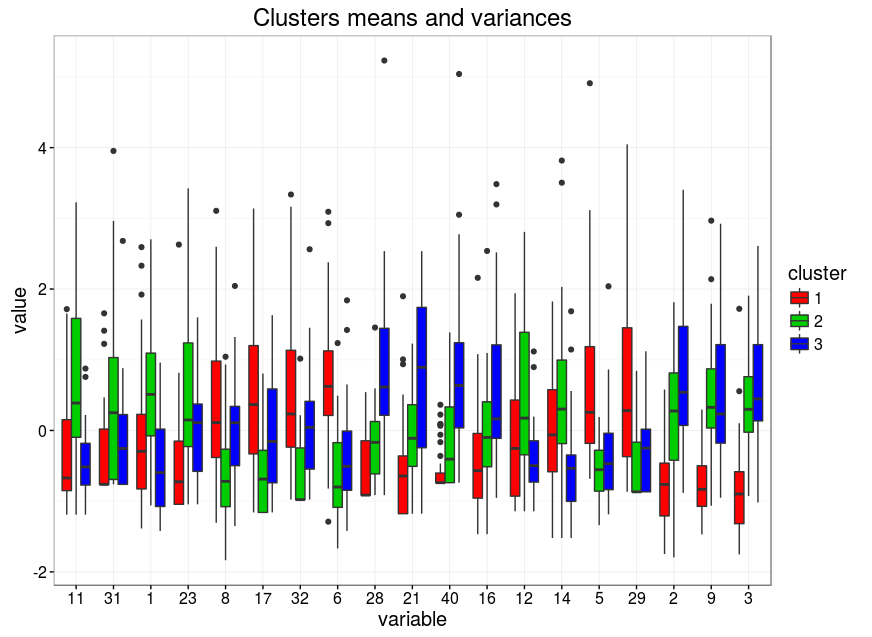
\includegraphics[width=0.5\textwidth]{whiskers}
	\caption{PCA projection of the clusters found and cluster profile in every dimension.}
	\label{fig:PCA}
\end{figure}

\subsection{Predictive roles}
One interesting use of roles is to make predictions on users behaviors. Here, we will analyze whether the initial composition of roles in a thread is a good predictor of the final length of the thread.

\section{Conclusions}
\bibliographystyle{spbasic} 
%\bibliographystyle{chicago} 
%\bibliographystyle{plainnat} 
\bibliography{library}
\end{document}